\documentclass[acmtog]{acmart}
\usepackage{graphicx}
\usepackage{subfigure}
\usepackage{natbib}
\usepackage{listings}
\usepackage{bm}
\usepackage{amsmath}

\definecolor{blve}{rgb}{0.3372549 , 0.61176471, 0.83921569}
\definecolor{gr33n}{rgb}{0.29019608, 0.7372549, 0.64705882}
\makeatletter
\lst@InstallKeywords k{class}{classstyle}\slshape{classstyle}{}ld
\makeatother
\lstset{language=C++,
	basicstyle=\ttfamily,
	keywordstyle=\radiance{blve}\ttfamily,
	stringstyle=\radiance{red}\ttfamily,
	commentstyle=\radiance{magenta}\ttfamily,
	morecomment=[l][\radiance{magenta}]{\#},
	classstyle = \bfseries\radiance{gr33n},
	tabsize=2
}
\lstset{basicstyle=\ttfamily}

% Title portion
\title{Assignment 4: {Global Illumination}}

\author{Name:\quad YIN HAIRUI  \\ student number:\ 2020533028
\\email:\quad yinhr@shanghaitech.edu.cn}

% Document starts
\begin{document}
\maketitle

\vspace*{2 ex}

\section{Introduction}
In this assignment, we are asked to render a scene by global illumination. Camera generates rays to pixel on the screen plane and ray intersects with objects. Considering ray tracing, we go through reflected rays sampled in each kind of object to the maximum depth. BRDF is our lighting model and Monte Carlo method is used to get a approximate value of BRDF. BVH structure is used for acceleration. \\ The followings are all jobs that have been done, including basic task and specular!
\begin{itemize}
	\item Path tracing with Monte Carlo integration: direct light and area light source
	\item Path tracing with Monte Carlo integration: indirect light
	\item Ideal diffuse BRDF
	\item Acceleration structure: BVH
	\item The ideal specular or glossy specular BRDF
\end{itemize}

\section{Implementation Details}
\subsection{Direct Light}
In traditional BRDF model, the radiance in the surface of object is composed by many weighted lights shooting to that point, where
$$L_o(x,\omega_o)=\int_{\Omega+}L_i(x,\omega_i)f_r(x,\omega_i, \omega_o)\cos{\theta}d\omega_i$$
To make it more simple, considering sampling light, we can rewrite the formula to:
$$L_o(x,\omega_o)=\int_{A}L_i(x,\omega_i)f_r(x,\omega_i, \omega_o)\frac{\cos{\theta}\cos{\theta'}}{||x'-x||^2}dA$$
Since the light in a position is mainly determined by the light source that shoots in, we can use the Monte Carlo form of the above formula to first calculate direct light, where Monte Carlo integration is as following:
$$L_o(p,\omega_o)\approx\frac{1}{N}\sum^N_{i=1}\frac{L_i(x,\omega_i)f_r(p,\omega_i,\omega_o)(n\cdot \omega_i)}{p(\omega_i)}$$
In this assignment, there is only one square light above, I use a uniform sample in the area, where $p=\frac{1}{area}$, so we get a sample on the light. The sample position and the object points generate a ray. After judging whether it is shadowed or not, if it is not shadowed, we pass the value calculated by  Monte Carlo integration to direct light value.
\subsection{Indirect Light}
After calculating the direct light, we are going to calculate the indirect light. Indirect light means light reflected or transmiited from other object which is not a light source. We first generate camera ray to the surface of an object, then find a ray which shoots from other object. With the loop method, we can trace the ray to a constant max depth, with Monte Carlo integration.
\subsection{Ideal diffuse BRDF}
The ideal diffuse is distributed uniformly, because we only trace one ray, I assume that the light is cos-weighted, with $p=\frac{1}{\pi}\cos{\theta}$, and the sample in a half unit sphere is as following:
$$\theta = \cos^{-1}(1-u_1)$$
$$\phi = 2 * \pi * u_2$$
$$x = \sin{\theta} * \cos{\phi}$$
$$y =\sin{\theta} * \sin{\phi}$$
$$z =\cos{\theta}$$
We get the instance "Interaction", then pass back the sampled direction into its composition "wi", and give its corresponding pdf when "IdealDiffusion::pdf" is used.
\subsection{BVH}
BVH is a tree structure used for dividing meshes into many small AABB structure. When we calculate intersection between meshes and ray, it is unnessary to traverse all meshes. Instead, we go through BVH to find which AABB bonding box intersects with the ray, iterate until the leaf node. The whole process reduces the meshes that is need for calculating intersection.\\
The core of the process is in the building of BVH and finding of which AABB boxes intersect with the ray. \\
In the building part, I calculate the center of each triangle of object, and find the Maximum span of axis. Selecting this axis as sorting standard and dividing the sorted triangles into left part and right part. And ensuring that the leaf node contains triangles less than "MAX\_LEAF\_SIZE".\\
In the intersection part, DFS the left and right node if the ray intersects with current node. All leaf nodes with AABB intersects with the ray are found, triangles inside are pushed out to do intersection test, and the intersecting point with the least distance is selected, stored into interaction variable.
\subsection{Specular}
The Specular inherits the same class of BSDF as Diffuse. Since it's ideal, the light shoot in is the reflect of the light shoot out, that is
$$\hat{R}_m=2(\hat{L}_m\cdot \hat{N})\hat{N}-\hat{L}_m$$
So the probability is $p=1$. And there is an addition part different from diffuse. Since we are using specular, it will reflect the light from light source even in indirect light. "isDelta" is used to distinguished whether the last ray comes from a specular object or diffuse object.
\section{Results}
The results are pictures following.\\
\begin{figure}[h]
	\centering
	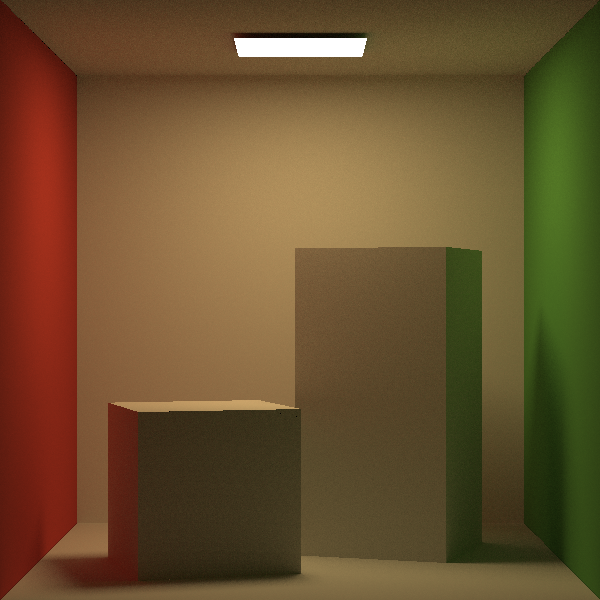
\includegraphics[width=0.7\linewidth]{simple.png}
	\caption{simple}
	\label{fig:simple}
\end{figure}
\begin{figure}[h]
	\centering
	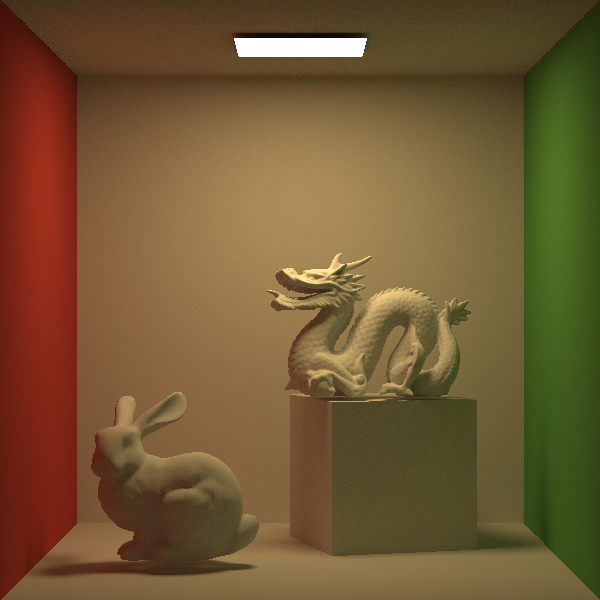
\includegraphics[width=0.7\linewidth]{BVH.png}
	\caption{Bunny and Dragon}
	\label{fig:BVH}
\end{figure}
\begin{figure}[h]
	\centering
	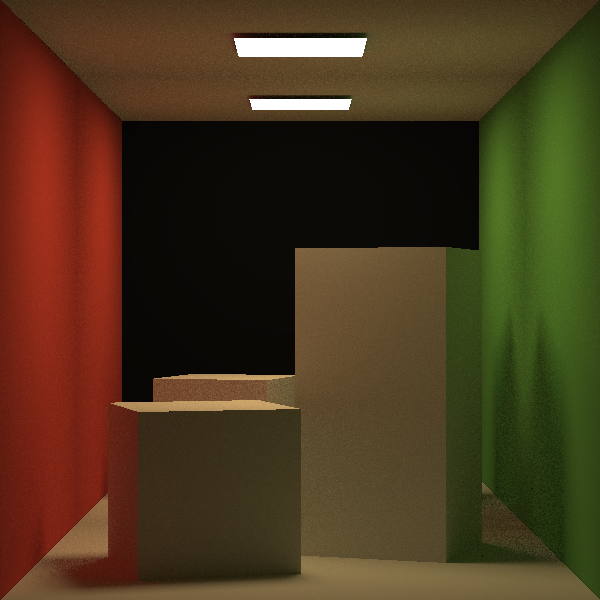
\includegraphics[width=0.7\linewidth]{Specular_back_900sample.png}
	\caption{Specular: back}
	\label{fig:BVH}
\end{figure}
\begin{figure}[h]
	\centering
	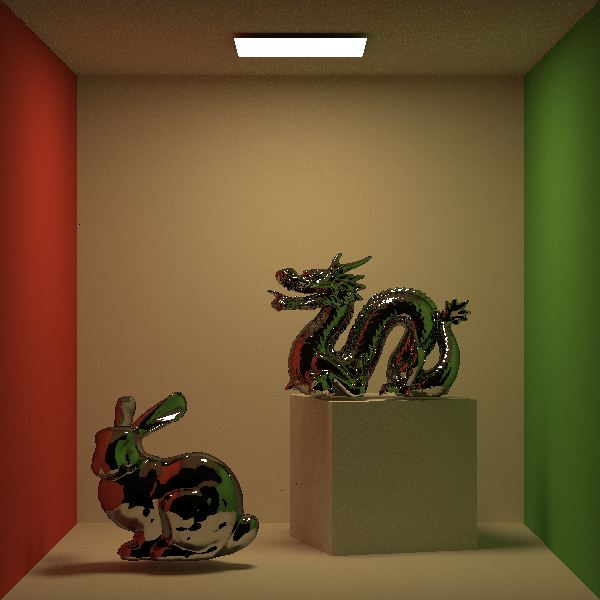
\includegraphics[width=0.7\linewidth]{Specular_bunnydragon.png}
	\caption{Specular: Bunny and Dragon}
	\label{fig:BVH}
\end{figure}

\end{document}
